\begin{enumerate}[label=\thesection.\arabic*,ref=\thesection.\theenumi]
\numberwithin{equation}{enumi}
\numberwithin{figure}{enumi}
\numberwithin{table}{enumi}
\item Determine if the points $(1,5),(2,3)$ and $(-2,-11)$ are collinear.
	\\
		\iffalse
\documentclass[12pt]{article}
\usepackage{graphicx}
\usepackage[none]{hyphenat}
\usepackage{graphicx}
\usepackage{listings}
\usepackage[english]{babel}
\usepackage{graphicx}
\usepackage{caption} 
\usepackage{hyperref}
\usepackage{booktabs}
\usepackage{array}
\usepackage{amsmath}   % for having text in math mode
\usepackage{extarrows} % for Row operations arrows
\usepackage{listings}
\lstset{
  frame=single,
  breaklines=true
}
  
%Following 2 lines were added to remove the blank page at the beginning
\usepackage{atbegshi}% http://ctan.org/pkg/atbegshi
\AtBeginDocument{\AtBeginShipoutNext{\AtBeginShipoutDiscard}}


%New macro definitions
\newcommand{\mydet}[1]{\ensuremath{\begin{vmatrix}#1\end{vmatrix}}}
\providecommand{\brak}[1]{\ensuremath{\left(#1\right)}}
\providecommand{\norm}[1]{\left\lVert#1\right\rVert}
\newcommand{\solution}{\noindent \textbf{Solution: }}
\newcommand{\myvec}[1]{\ensuremath{\begin{pmatrix}#1\end{pmatrix}}}
\let\vec\mathbf

\begin{document}

\begin{center}
\title{\textbf{Properties of Triangles}}
\date{\vspace{-5ex}} %Not to print date automatically
\maketitle
\end{center}
\setcounter{page}{1}

\section{10$^{th}$ Maths - Chapter 7}
This is Problem-3 from Exercise 7.1
\begin{enumerate}
\item Determine if the points $(1,5), (2,3), \text{ and } (-2,-11)$ are collinear.  \\
	\fi
\solution 
 We know that points $\vec{A}, \vec{B} \text{ and } \vec{C}$ are collinear, if
\begin{align}
  \label{eq:10/7/1/31}
\text{rank}\myvec{ 
	\vec{A}^\top \\ 
	\vec{B}^\top \\ 
	\vec{C}^\top 
}    &=  1 
\end{align}
Since
\begin{align}
	\myvec{ \vec{A}^\top \\ 
			\vec{B}^\top \\ 
			\vec{C}^\top 
} =   		\myvec{
        		1 & 5 \\
        		2 & 3 \\
        		-2 & -11 
}
\\
\xleftrightarrow[{R_3\rightarrow R_3+2R_1}]{{R_2\rightarrow R_2-2R_1}}  \myvec{
  1 & 5 \\
  0 & -7 \\
  0 & -1 
}    
\xleftrightarrow[]{{R_3\rightarrow R_3-\frac{1}{7}R_2}}  \myvec{
  1 & 5 \\
  0 & -7 \\
  0 & 0 
},
\end{align}
 the rank of the matrix is 2. From \eqref{eq:10/7/1/31}, the points are not collinear.  This is verified by Fig.  
 \ref{fig:10/7/1/3Fig1}, where the given points constitute a triangle and not a line.
\begin{figure}[!h]
	\begin{center}
		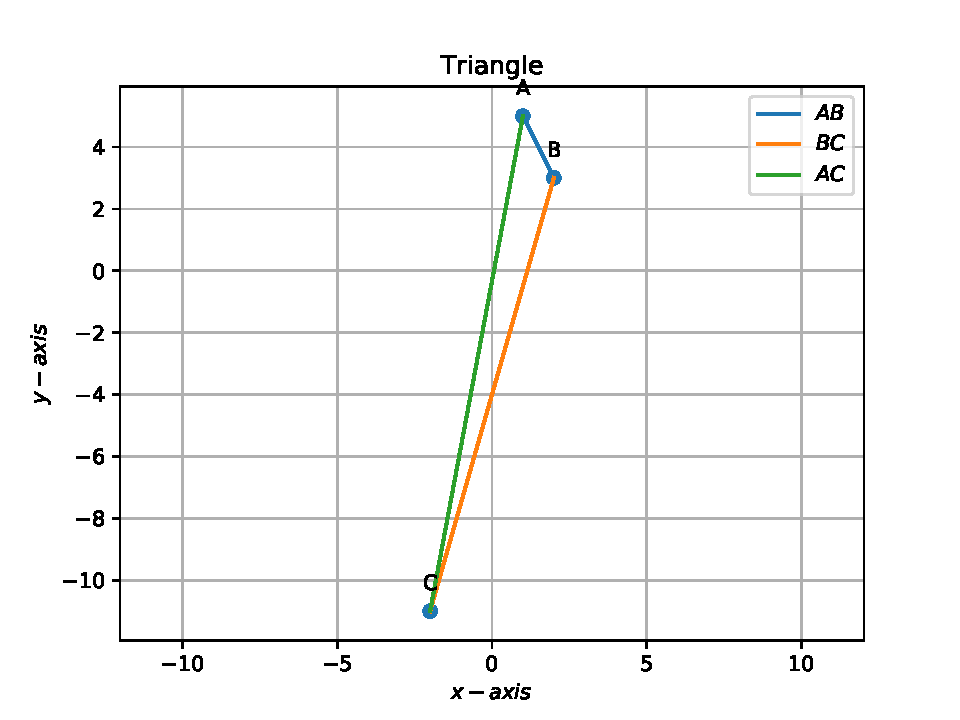
\includegraphics[width=\columnwidth]{chapters/10/7/1/3/figs/problem3.pdf}
	\end{center}
\caption{}
\label{fig:10/7/1/3Fig1}
\end{figure}


\item Show that the points $\vec{A}(1,2,7), \vec{B}(2,6,3)$ and $\vec{C}(3,10,-1)$ are collinear.
	\\
	\solution
		\iffalse
\documentclass[journal,12pt,twocolumn]{IEEEtran}
\usepackage{setspace}
\usepackage{gensymb}
\usepackage{xcolor}
\usepackage{caption}
\singlespacing
\usepackage{siunitx}
\usepackage[cmex10]{amsmath}
\usepackage{mathtools}
\usepackage{hyperref}
\usepackage{amsthm}
\usepackage{mathrsfs}
\usepackage{txfonts}
\usepackage{stfloats}
\usepackage{cite}
\usepackage{cases}
\usepackage{subfig}
\usepackage{longtable}
\usepackage{multirow}
\usepackage{enumitem}
\usepackage{mathtools}
\usepackage{listings}
\usepackage{tikz}
\usetikzlibrary{shapes,arrows,positioning}
\usepackage{circuitikz}
\let\vec\mathbf
\DeclareMathOperator*{\Res}{Res}
\renewcommand\thesection{\arabic{section}}
\renewcommand\thesubsection{\thesection.\arabic{subsection}}
\renewcommand\thesubsubsection{\thesubsection.\arabic{subsubsection}}

\renewcommand\thesectiondis{\arabic{section}}
\renewcommand\thesubsectiondis{\thesectiondis.\arabic{subsection}}
\renewcommand\thesubsubsectiondis{\thesubsectiondis.\arabic{subsubsection}}
\hyphenation{op-tical net-works semi-conduc-tor}

\lstset{
language=Python,
frame=single, 
breaklines=true,
columns=fullflexible
}
\begin{document}
\theoremstyle{definition}
\newtheorem{theorem}{Theorem}[section]
\newtheorem{problem}{Problem}
\newtheorem{proposition}{Proposition}[section]
\newtheorem{lemma}{Lemma}[section]
\newtheorem{corollary}[theorem]{Corollary}
\newtheorem{example}{Example}[section]
\newtheorem{definition}{Definition}[section]
\newcommand{\BEQA}{\begin{eqnarray}}
\newcommand{\EEQA}{\end{eqnarray}}
\newcommand{\define}{\stackrel{\triangle}{=}}
\newcommand{\myvec}[1]{\ensuremath{\begin{pmatrix}#1\end{pmatrix}}}
\newcommand{\mydet}[1]{\ensuremath{\begin{vmatrix}#1\end{vmatrix}}}
\bibliographystyle{IEEEtran}
\providecommand{\nCr}[2]{\,^{#1}C_{#2}} % nCr
\providecommand{\nPr}[2]{\,^{#1}P_{#2}} % nPr
\providecommand{\mbf}{\mathbf}
\providecommand{\pr}[1]{\ensuremath{\Pr\left(#1\right)}}
\providecommand{\qfunc}[1]{\ensuremath{Q\left(#1\right)}}
\providecommand{\sbrak}[1]{\ensuremath{{}\left[#1\right]}}
\providecommand{\lsbrak}[1]{\ensuremath{{}\left[#1\right.}}
\providecommand{\rsbrak}[1]{\ensuremath{{}\left.#1\right]}}
\providecommand{\brak}[1]{\ensuremath{\left(#1\right)}}
\providecommand{\lbrak}[1]{\ensuremath{\left(#1\right.}}
\providecommand{\rbrak}[1]{\ensuremath{\left.#1\right)}}
\providecommand{\cbrak}[1]{\ensuremath{\left\{#1\right\}}}
\providecommand{\lcbrak}[1]{\ensuremath{\left\{#1\right.}}
\providecommand{\rcbrak}[1]{\ensuremath{\left.#1\right\}}}
\theoremstyle{remark}
\newtheorem{rem}{Remark}
\newcommand{\sgn}{\mathop{\mathrm{sgn}}}
\newcommand{\rect}{\mathop{\mathrm{rect}}}
\newcommand{\sinc}{\mathop{\mathrm{sinc}}}
\providecommand{\abs}[1]{\left\vert#1\right\vert}
\providecommand{\res}[1]{\Res\displaylimits_{#1}} 
\providecommand{\norm}[1]{\lVert#1\rVert}
\providecommand{\mtx}[1]{\mathbf{#1}}
\providecommand{\mean}[1]{E\left[ #1 \right]}
\providecommand{\fourier}{\overset{\mathcal{F}}{ \rightleftharpoons}}
\providecommand{\ztrans}{\overset{\mathcal{Z}}{ \rightleftharpoons}}
\providecommand{\system}[1]{\overset{\mathcal{#1}}{ \longleftrightarrow}}
\newcommand{\solution}{\noindent \textbf{Solution: }}
\providecommand{\dec}[2]{\ensuremath{\overset{#1}{\underset{#2}{\gtrless}}}}
\let\StandardTheFigure\thefigure
\def\putbox#1#2#3{\makebox[0in][l]{\makebox[#1][l]{}\raisebox{\baselineskip}[0in][0in]{\raisebox{#2}[0in][0in]{#3}}}}
     \def\rightbox#1{\makebox[0in][r]{#1}}
     \def\centbox#1{\makebox[0in]{#1}}
     \def\topbox#1{\raisebox{-\baselineskip}[0in][0in]{#1}}
     \def\midbox#1{\raisebox{-0.5\baselineskip}[0in][0in]{#1}}

\vspace{3cm}
\title{Line Assignment}
\author{Gautam Singh}
\maketitle
\bigskip

\begin{abstract}
    This document contains the solution to Question 16 of Exercise 3 in Chapter
    10 of the class 12 NCERT textbook.
\end{abstract}

\begin{enumerate}
    \item Show that the points $\vec{A} = \myvec{1\\2\\7}$, $\vec{B} = 
    \myvec{2\\6\\3}$, and $\vec{C} = \myvec{3\\10\\-1}$ are collinear.


    \solution 
\fi
		Points $\vec{A}$, $\vec{B}$ and $\vec{C}$ are on a line if
    \begin{align}
        \textrm{rank}\myvec{\vec{A} & \vec{B} & \vec{C}} < 3
        \label{eq:chapters/12/10/3/16rank-collinear}
    \end{align}
    Substituting, we must find the rank of
    \begin{align}
        \vec{M} = \myvec{1&2&3\\2&6&10\\7&3&-1}
    \end{align}
    Using row reduction methods to bring $\mtx{M}$ into row-reduced echelon
    form,
    \begin{align}
        \myvec{1&2&3\\2&6&10\\7&3&-1}&\xleftrightarrow[]{R_2\rightarrow R_2-2R_1}
        \myvec{1&2&3\\0&2&4\\7&3&-1} \\
                &\xleftrightarrow[]{R_3\rightarrow R_3-7R_1}\myvec{1&2&3\\0&2&4\\0&-11&-22} \\
                &\xleftrightarrow[]{R_1\rightarrow R_1-R_2}\myvec{1&0&-1\\0&2&4\\0&-11&-22} \\
                &\xleftrightarrow[]{R_3\rightarrow R_3+\frac{11}{2}R_2}\myvec{1&0&-1\\0&2&4\\0&0&0}
                \label{eq:chapters/12/10/3/16row-red}
    \end{align}
    Clearly, the rank of $\mtx{M}$ is 2, and hence the given points are 
    collinear. 
    Fig. \ref{fig:chapters/12/10/3/163d-line}  verifies that the three points are indeed 
    collinear as claimed.
    \begin{figure}[!ht]
        \centering
        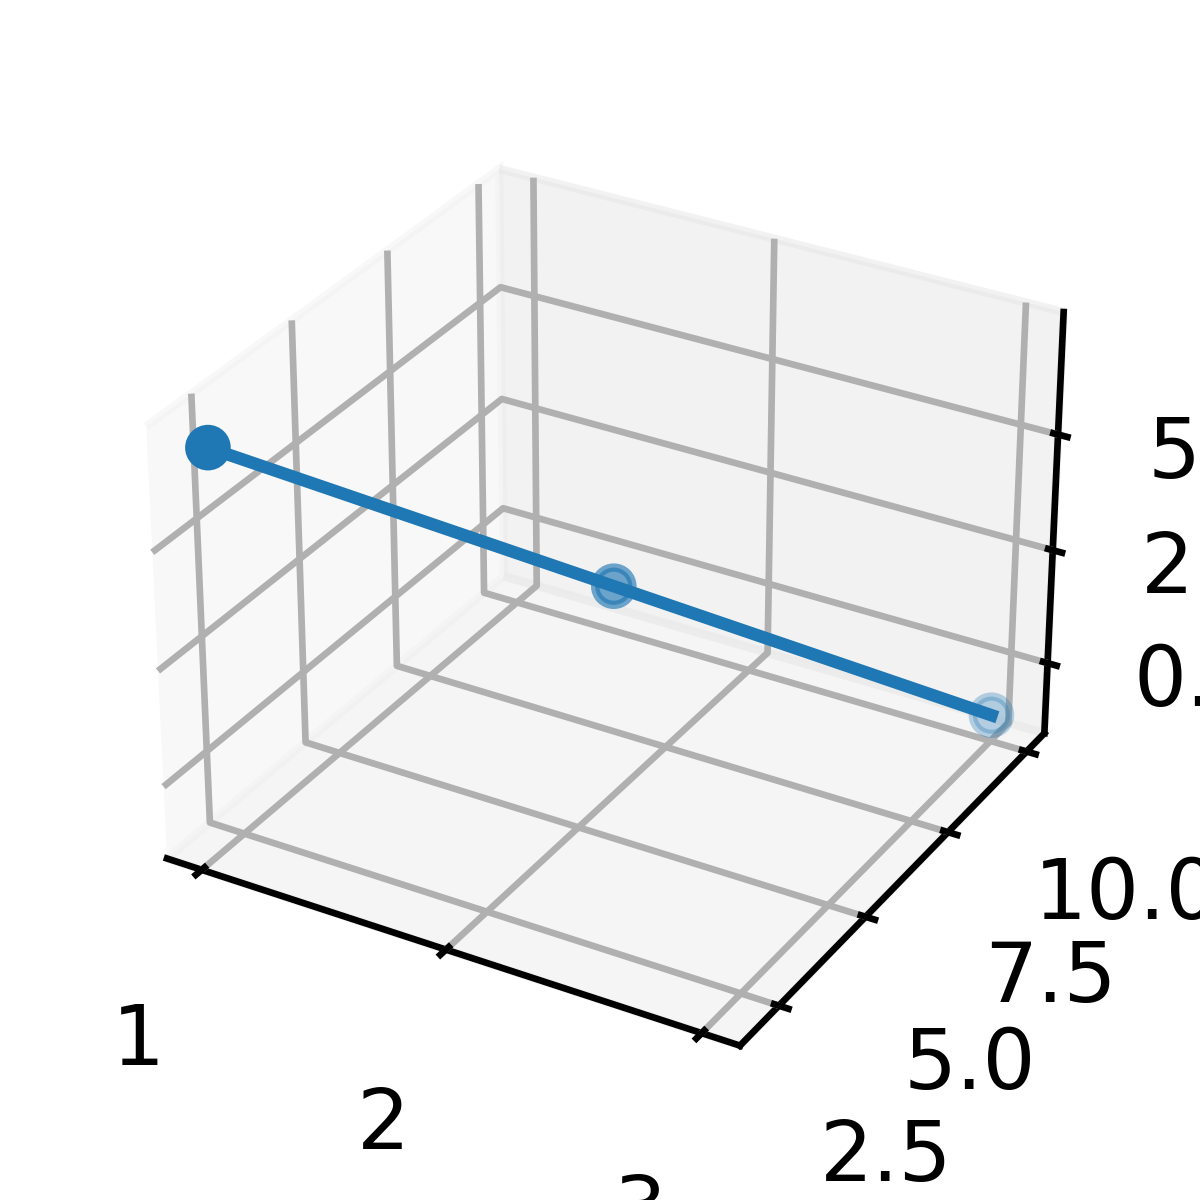
\includegraphics[width=\columnwidth]{chapters/12/10/3/16/figs/line_3d.png}
        \caption{Points $\vec{A}$, $\vec{B}$ and $\vec{C}$ are collinear.}
        \label{fig:chapters/12/10/3/163d-line}
    \end{figure}

\item Show that the vectors $2\hat{i}-3\hat{j}+4\hat{k}$ and $-4\hat{i}+6\hat{j}-8\hat{k}$ are collinear.
   \\ 
    \solution 
		\iffalse
\documentclass[12pt]{article}
\usepackage{graphicx}
\graphicspath{{./figs/}}{}
\usepackage{amsmath,amssymb,amsfonts,amsthm}
\newcommand{\myvec}[1]{\ensuremath{\begin{pmatrix}#1\end{pmatrix}}}
\providecommand{\norm}[1]{\lVert#1\rVert}
\usepackage{listings}
\usepackage{watermark}
\usepackage{titlesec}
\usepackage{caption}
\usepackage{extarrows}
\let\vec\mathbf
\lstset{
frame=single, 
breaklines=true,
columns=fullflexible
}
\thiswatermark{\centering \put(0,-105.0){
\includegraphics[scale=0.15]{/sdcard/IITH/vectors/12.10.2.11/figs/logo.png}} }
\title{\mytitle}
\title{
Assignment - 12.10.2.11
}
\author{Surajit Sarkar}
\begin{document}
\maketitle
\tableofcontents
\bigskip
\section{\textbf{Problem}}
Show that the vectors $2\hat{i}+3\hat{j}+4\hat{k}$ and $-4\hat{i}+6\hat{j}-8\hat{k}$ are collinear.
\section{\textbf{Solution}}
\fi
Let
\begin{align}
\vec{A}=\myvec{2\\3\\4},\vec{B}=\myvec{-4\\6\\-8}\\
 \end{align}
 Forming the collinearity matrix
 \begin{align}        
\myvec{\vec{A}^{\top}\\ \vec{B}^{\top}}=\myvec{2&-3&4\\-4&6&-8}
 \xleftrightarrow{\frac{1}{2}R_1\to R_1}\myvec{1&-\frac{3}{2}&2\\-4&6&-8}\\
\xleftrightarrow{-\frac{1}{4}R_2\leftarrow R_2}\myvec{1&-\frac{3}{2}&2\\1&\frac{3}{2}&2}
\xleftrightarrow{R_2-1R_1\to R_2}\myvec{1&-\frac{3}{2}&2\\0&0&0}
\end{align}
Thus, the rank of the matrix is 1 and the vectors are collinear.

\item Show that the points (2, 3, 4), (–1, –2, 1), (5, 8, 7) are collinear.
		\\
		\solution
		\iffalse
\documentclass[journal,12pt,twocolumn]{IEEEtran}
\usepackage{setspace}
\usepackage{gensymb}
\singlespacing
\usepackage[cmex10]{amsmath}
\usepackage{amsthm}
\usepackage{mathrsfs}
\usepackage{txfonts}
\usepackage{stfloats}
\usepackage{bm}
\usepackage{cite}
\usepackage{cases}
\usepackage{subfig}
\usepackage{longtable}
\usepackage{multirow}
\usepackage{enumitem}
\usepackage{mathtools}
\usepackage{steinmetz}
\usepackage{tikz}
\usepackage{circuitikz}
\usepackage{verbatim}
\usepackage{tfrupee}
\usepackage[breaklinks=true]{hyperref}
\usepackage{tkz-euclide}
\usetikzlibrary{calc,math}
\usepackage{listings}
    \usepackage{color}                                            %%
    \usepackage{array}                                            %%
    \usepackage{longtable}                                        %%
    \usepackage{calc}                                             %%
    \usepackage{multirow}                                         %%
    \usepackage{hhline}                                           %%
    \usepackage{ifthen}                                           %%
  %optionally (for landscape tables embedded in another document): %%
    \usepackage{lscape}     
\usepackage{multicol}
\usepackage{chngcntr}
\DeclareMathOperator*{\Res}{Res}
\renewcommand\thesection{\arabic{section}}
\renewcommand\thesubsection{\thesection.\arabic{subsection}}
\renewcommand\thesubsubsection{\thesubsection.\arabic{subsubsection}}

\renewcommand\thesectiondis{\arabic{section}}
\renewcommand\thesubsectiondis{\thesectiondis.\arabic{subsection}}
\renewcommand\thesubsubsectiondis{\thesubsectiondis.\arabic{subsubsection}}

% correct bad hyphenation here
\hyphenation{op-tical net-works semi-conduc-tor}
\def\inputGnumericTable{}                                 %%

\lstset{
frame=single, 
breaklines=true,
columns=fullflexible
}

\begin{document}


\newtheorem{theorem}{Theorem}[section]
\newtheorem{problem}{Problem}
\newtheorem{proposition}{Proposition}[section]
\newtheorem{lemma}{Lemma}[section]
\newtheorem{corollary}[theorem]{Corollary}
\newtheorem{example}{Example}[section]
\newtheorem{definition}[problem]{Definition}
\newcommand{\BEQA}{\begin{eqnarray}}
\newcommand{\EEQA}{\end{eqnarray}}
\newcommand{\define}{\stackrel{\triangle}{=}}

\bibliographystyle{IEEEtran}
\providecommand{\mbf}{\mathbf}
\providecommand{\pr}[1]{\ensuremath{\Pr\left(#1\right)}}
\providecommand{\qfunc}[1]{\ensuremath{Q\left(#1\right)}}
\providecommand{\sbrak}[1]{\ensuremath{{}\left[#1\right]}}
\providecommand{\lsbrak}[1]{\ensuremath{{}\left[#1\right.}}
\providecommand{\rsbrak}[1]{\ensuremath{{}\left.#1\right]}}
\providecommand{\brak}[1]{\ensuremath{\left(#1\right)}}
\providecommand{\lbrak}[1]{\ensuremath{\left(#1\right.}}
\providecommand{\rbrak}[1]{\ensuremath{\left.#1\right)}}
\providecommand{\cbrak}[1]{\ensuremath{\left\{#1\right\}}}
\providecommand{\lcbrak}[1]{\ensuremath{\left\{#1\right.}}
\providecommand{\rcbrak}[1]{\ensuremath{\left.#1\right\}}}
\theoremstyle{remark}
\newtheorem{rem}{Remark}
\newcommand{\sgn}{\mathop{\mathrm{sgn}}}
\providecommand{\abs}[1]{\left\vert#1\right\vert}
\providecommand{\res}[1]{\Res\displaylimits_{#1}} 
\providecommand{\norm}[1]{\left\lVert#1\right\rVert}
\providecommand{\mtx}[1]{\mathbf{#1}}
\providecommand{\mean}[1]{E\left[ #1 \right]}
\providecommand{\fourier}{\overset{\mathcal{F}}{ \rightleftharpoons}}
\providecommand{\system}{\overset{\mathcal{H}}{ \longleftrightarrow}}
\newcommand{\solution}{\noindent \textbf{Solution: }}
\newcommand{\cosec}{\,\text{cosec}\,}
\providecommand{\dec}[2]{\ensuremath{\overset{#1}{\underset{#2}{\gtrless}}}}
\newcommand{\myvec}[1]{\ensuremath{\begin{pmatrix}#1\end{pmatrix}}}
\newcommand{\mydet}[1]{\ensuremath{\begin{vmatrix}#1\end{vmatrix}}}
\numberwithin{equation}{subsection}
\makeatletter
\@addtoreset{figure}{problem}
\makeatother

\let\StandardTheFigure\thefigure
\let\vec\mathbf
\renewcommand{\thefigure}{\theproblem}



\def\putbox#1#2#3{\makebox[0in][l]{\makebox[#1][l]{}\raisebox{\baselineskip}[0in][0in]{\raisebox{#2}[0in][0in]{#3}}}}
     \def\rightbox#1{\makebox[0in][r]{#1}}
     \def\centbox#1{\makebox[0in]{#1}}
     \def\topbox#1{\raisebox{-\baselineskip}[0in][0in]{#1}}
     \def\midbox#1{\raisebox{-0.5\baselineskip}[0in][0in]{#1}}

\vspace{3cm}


\title{Assignment 1}
\author{Jaswanth Chowdary Madala}





% make the title area
\maketitle

\newpage

%\tableofcontents

\bigskip

\renewcommand{\thefigure}{\theenumi}
\renewcommand{\thetable}{\theenumi}


\begin{enumerate}


\textbf{Solution:} 
\fi
		The points given are,
\begin{align}
\vec{A} = \myvec{2\\3\\4}, \, \vec{B} = \myvec{-1\\-2\\1}, \,\vec{C}=\myvec{5\\8\\7}
\end{align}
%
To check whether the given points are collinear, we find the rank of the matrix 
%
\begin{align}
\myvec{\vec{A} & \vec{B} & \vec{C}}
=\myvec{2&-1&5\\3&-2&8\\4&1&7}
\xleftrightarrow[R_3 \leftarrow R_3 - 2R_1]{R_2 \leftarrow R_2 - \frac{3}{2}R_1}
\myvec{2&-1&5\\ \\0&-\frac{1}{2}&\frac{1}{2}\\ \\0&3&-3}\\
\xleftrightarrow{R_3 \leftarrow R_3 + 6R_2}
\myvec{2&-1&5\\\\0&-\frac{1}{2}&\frac{1}{2}\\\\0&0&0}
\end{align}
The matrix has a rank of 2. Hence the given points are collinear.




\item In each of the following, find the value of '$k$', for which the points are collinear.
\begin{enumerate}
\item $(7, –2), (5, 1), (3, k)$
\item $(8, 1), (k, – 4), (2, –5)$
\end{enumerate}
		\label{10/7/3/2}
\solution
		\iffalse
\documentclass[journal,10pt,twocolumn]{article}
\usepackage{graphicx}
\usepackage{caption} 
\usepackage{hyperref}
\usepackage[margin=0.5in]{geometry}
\usepackage{booktabs}
\usepackage{array}
\usepackage{amsmath}   % for having text in math mode
\usepackage{mathtools}
\usepackage{enumitem}
\usepackage{atbegshi}% http://ctan.org/pkg/atbegshi
\AtBeginDocument{\AtBeginShipoutNext{\AtBeginShipoutDiscard}}
\newcommand{\myvec}[1]{\ensuremath{\begin{pmatrix}#1\end{pmatrix}}}
\let\vec\mathbf
\newcommand{\mydet}[1]{\ensuremath{\begin{vmatrix}#1\end{vmatrix}}}
\providecommand{\brak}[1]{\ensuremath{\left(#1\right)}}
\newcommand{\solution}{\noindent \textbf{Solution: }}
\let\vec\mathbf
\begin{document}
\begin{center}
\title{\textbf{Properties of Collinear}}
\date{\vspace{-5ex}} %Not to print date automatically
\maketitle
\end{center}
\setcounter{page}{1}
\section{10$^{th}$ Maths - Chapter 7}
\textbf{This is Problem-2 from Exercise 7.3.2}
\item In each of the following find the value of ‘k’, for which the points are collinear.

\item (7, –2), (5, 1), (3, k) \\
\item (8, 1), (k, – 4), (2, –5).\\
\fi
\begin{enumerate}
\item 
Let
\begin{align}  
	\vec{A}&=\myvec{7 \\-2},
\vec{B}=\myvec{5 \\ 1},
\vec{C}=\myvec{3 \\ k}
\end{align}
Then
\begin{align}  
\vec{D} &=\brak{\vec{A}-\vec{B}} = \brak{\myvec{7 \\-2 } - \myvec{5 \\1 } } = \myvec{2 \\ -3 }\\
\vec{E} &= \brak{\vec{A}-\vec{C}} = \brak{\myvec{7 \\ -2 } - \myvec{3 \\k} } = \myvec{4 \\-2-k}
\end{align}
Forming the collinearlity matrix,
\begin{align}
\vec{F} &={\myvec{\vec{D}\\ \vec{E}}}
=
\myvec{
2 & -3
 \\
4 & -2-k 
}
\end{align}
yielding
\begin{align}
\label{eq:chapters/10/7/3/2/chem_balance_mat_row1}
 \xleftrightarrow[]{R_2 = R_2-2R_1}
\myvec{
2 & -3
\\
0 & -k+4
}
\end{align}
For the matrix to be rank 1, 
\begin{align}
 -k+4 =0
\implies k =4 
\end{align}
This is verified in Fig. 
	  \ref{fig:chapters/10/7/3/2/line1.pdf}.
\begin{figure}[h!]
	  \centering 
	  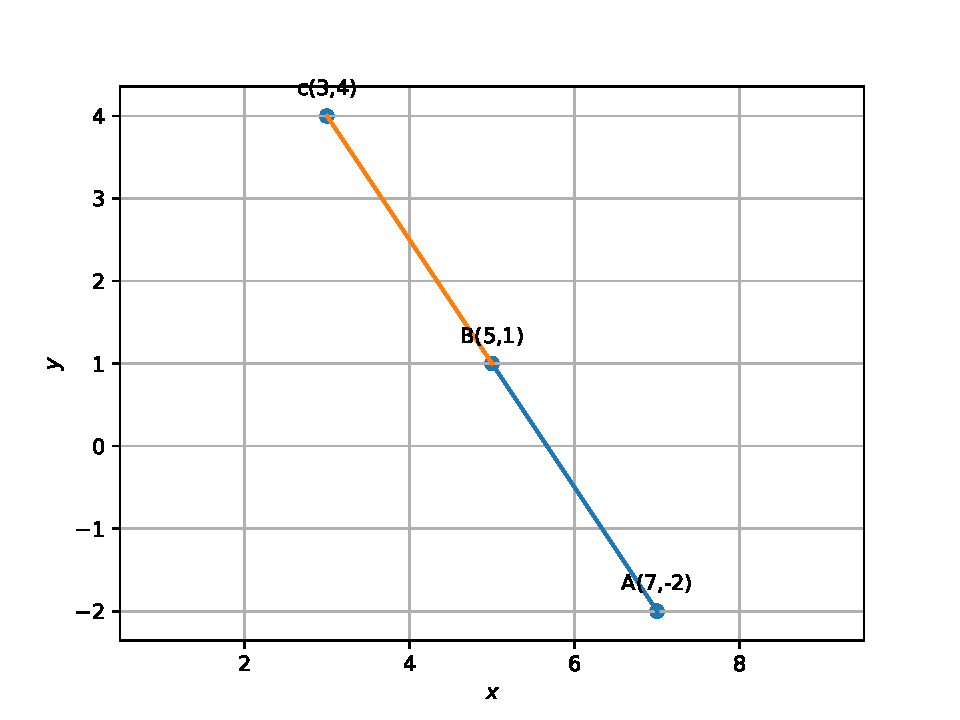
\includegraphics[width=\columnwidth]{chapters/10/7/3/2/figs/line1.pdf}
	  \caption{}
	  \label{fig:chapters/10/7/3/2/line1.pdf}
	  \end{figure} 	 		  
%
 \item In this case,
\begin{align}  
\vec{A}=\myvec{8 \\ 1},
\vec{B}=\myvec{k \\ -4},
\vec{C}=\myvec{2 \\ -5}.
\end{align}
Since
\begin{align}  
 \vec{D} &=\brak{\vec{A}-\vec{B}} = \brak{\myvec{8 \\1 } - \myvec{k \\-4 } } = \myvec{8-k \\ 5 }\\
\vec{E} &= \brak{\vec{A}-\vec{C}} = \brak{\myvec{8 \\ 1 } - \myvec{2 \\-5 } } = \myvec{6 \\6}
\end{align}
the collinearity matrix is
\begin{align}
\vec{F} &={\myvec{\vec{D}\\ \vec{E}}}
=
\myvec{
8-k & 5
 \\
6 & 6
}
\end{align}
yielding
\begin{align}
\label{eq:chapters/10/7/3/2/chem_balance_mat_row}
 \xleftrightarrow[]{R_1=\frac{R_1}{8-k}}
\myvec{
1& \frac{5}{8-k}
\\
6 & 6
}
\\
\xleftrightarrow[]{R_2 = R_2-6R_1}
\myvec{
1 & \frac{5}{8-k}
\\
\\
0 & 6-\frac{30}{8-k}
}
\end{align}
For 
the matrix to be rank 1,
\begin{align}
6-\frac{30}{8-k}&=0
\\
\implies k &=3
\end{align}
This is verified in Fig. 
	  \ref{fig:chapters/10/7/3/2/line2.png}
\begin{figure}[h]
	  \centering 
	  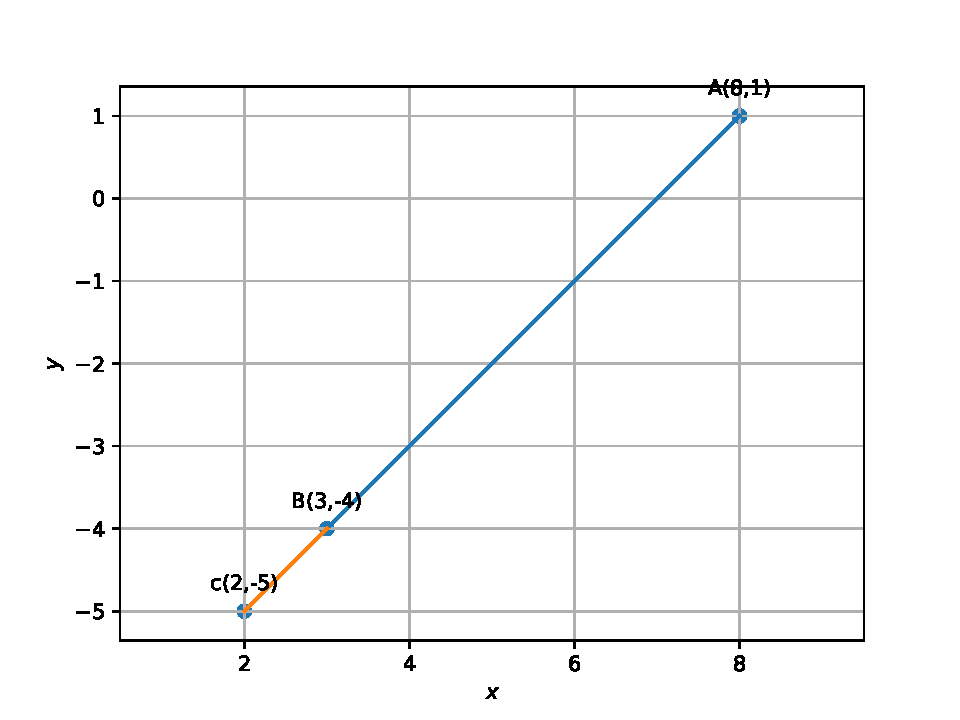
\includegraphics[width=\columnwidth]{chapters/10/7/3/2/figs/line2.pdf}
	  \caption{}
	  \label{fig:chapters/10/7/3/2/line2.png}
	  \end{figure}
\end{enumerate} 

\item Find a relation between $x$ and $y$ if the points $(x, y), (1, 2)$  and  $(7, 0)$ are collinear.
\\
\solution
	\iffalse
\documentclass[12pt]{article}
\usepackage{graphicx}
\usepackage{amsmath}
\usepackage{mathtools}
\usepackage{gensymb}

\newcommand{\mydet}[1]{\ensuremath{\begin{vmatrix}#1\end{vmatrix}}}
\providecommand{\brak}[1]{\ensuremath{\left(#1\right)}}
\providecommand{\norm}[1]{\left\lVert#1\right\rVert}
\newcommand{\solution}{\noindent \textbf{Solution: }}
\newcommand{\myvec}[1]{\ensuremath{\begin{pmatrix}#1\end{pmatrix}}}
\let\vec\mathbf

\begin{document}
\begin{center}
\textbf\large{CHAPTER-7 \\ COORDINATE GEOMETRY}
\end{center}
\section*{Excercise 7.4}

Q2. Find a relation between x and y if the points $\vec(x, y), \vec(1, 2) \text{ and } \vec(7, 0)$ are collinear.
\\
\solution
\\
The coordinates are given as
\fi
Let
	\begin{align}
	\vec{A} = \myvec{
		x\\
		y\\
		},
	\vec{B} = \myvec{
		1\\
		2\\
		},
	\vec{C} = \myvec{
		7\\
		0\\
		}
	\end{align}
	Then
	\begin{align}
\vec{D} &=\brak{\vec{A}-\vec{B}} = \brak{\myvec{x \\y } - \myvec{1 \\2 } } = \myvec{x-1 \\ y-2 }\\
\vec{E} &= \brak{\vec{A}-\vec{C}} = \brak{\myvec{x \\ y } - \myvec{7 \\0} } = \myvec{x-7 \\y}
\end{align}
Forming the collinearity matrix
\begin{align}
	\vec{F} &={\myvec{\vec{D}^{\top}\\ \vec{E}^{\top}}}
\end{align}
and performing row reduction,
\begin{align}
\label{eq:chapters/10/7/4/2chem_balance_mat_row}
\myvec{
x-1 & y-2
\\
x-7 & y
}
\xleftrightarrow[]{R_2 = R_2-R_1}
\myvec{
  x-1 & y-2
  \\
	  -6 & 2                 
	  }
	  \\
	\xleftrightarrow[]{R_2 = \frac{R_2}{-6}(x-1)-R_1}
\myvec{
x-1 & y-2
\\
	0 & -\frac{1}{3}(x-1)-(y-2)
}
\end{align}
For the rank of the matrix to be 1,
\begin{align}
	-\frac{1}{3}(x-1)-(y-2)&=0\\
	\implies \myvec{1 & 3}\vec{x} &=7	
\end{align}
For $x=-2, y=3$, see Fig. \ref{fig:chapters/10/7/4/2Fig} verifying that the points are collinear.
\begin{figure}[!h]
	\begin{center} 
	    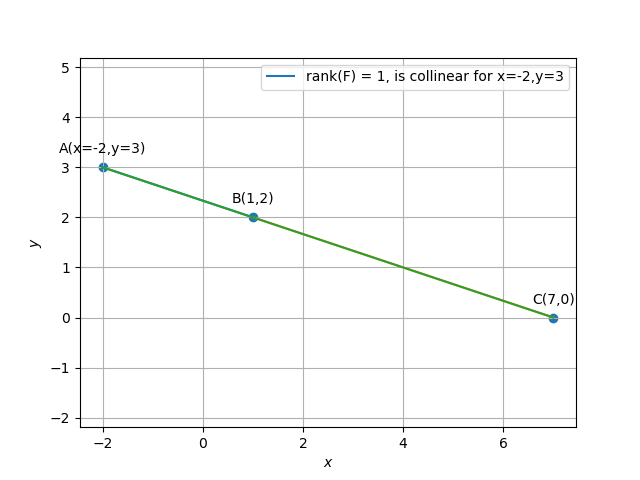
\includegraphics[width=\columnwidth]{chapters/10/7/4/2/figs/sc1.png}
	\end{center}
\caption{}
\label{fig:chapters/10/7/4/2Fig}
\end{figure}

\item If three points $(x, -1), (2, 1)$ and $(4, 5)$ are collinear, find the value of $x$.
\label{chapters/11/10/1/8}
\iffalse
\documentclass[10pt, a4paper]{article}
\usepackage[a4paper,outer=1.5cm,inner=1.5cm,top=1.75cm,bottom=1.5cm]{geometry}

\twocolumn
\usepackage{graphicx}

\usepackage{hyperref}
\usepackage[utf8]{inputenc}
\usepackage{amsmath}
\usepackage{physics}
\usepackage{amssymb}
\begin{document}
\title{Assignment-4}
\author{Name:C.CHANDANA\and Email :  \url{cheenepallichandana531@gmail.com}}
%\{ Wireless Communication (FWC)}
\date{30-sep-2022}
\maketitle



\section{Problem}
\fi
If three points $(x, -1), (2, 1)$ and $(4, 5)$ are collinear, find the value of $x$.
\\
\solution 
	\begin{figure}[!ht]
		\centering
 \includegraphics[width=\columnwidth]{chapters/11/10/1/8/figs/sline.png}
		\caption{}
		\label{fig:11/10/1/8}
  	\end{figure}
	\iffalse
\begin{center}
	\fi
	Let
\begin{align} \label{eq:11/10/1/8}
	\vec{A}=\myvec{ x\\ -1 },
	\vec{B}=\myvec{ 2\\ 1 },
\vec{C}=\myvec{ 4\\ 5 }.
\end{align}
Then
\begin{align}
\vec{A}-\vec{B}
	&=\myvec{ x-2\\ -2 }
	\\
\vec{A}-\vec{C}
	&=\myvec{ 4-x\\ 6 }
\end{align}
Forming the collinearity matrix
using 
	\eqref{eq:normal_line-collinear},
\begin{align} 
\myvec{ x-2 & -2\\ 4-x & 6  } 
	\xleftrightarrow[]{{R_1=3R_1+R-2}}
=\myvec{
2x-2 &0 \\ 
 4-x& 6
}
\end{align}

\iffalse

In the problem they have given that three points lie on a line, thats means these three points are collinear.\\

If  points on a line  are  collinear, rank of matrix is " 1 "then the vectors are in linearlydependent.\\
For 2 × 2 matrix Rank =1 means Determinant is 0.\\

Through pivoting,we obtain\\
\begin{align}
=\myvec{ x-2 & -2\\ 4-x & 6 \ } \\ 
\end{align}
\begin{align}
=\myvec{
x-2 &-2 \\ 
 4-x& 6
}\overset{R1=3R1+R2}{\rightarrow}
=\myvec{
2x-2 &0 \\ 
 4-x& 6
}
\end{align} 
\fi
	If the rank of the matrix is 1, any one of the rows must be zero. So, making the first element in the above matrix 0,
\begin{align}
x=1
\end{align} 

\iffalse

\begin{align}\label{eq:11/10/1/8}
x=1 \\
\end{align} 

Hence proved.\\
\section{Construction}
 \begin{figure}[h]
\centering
\includegraphics[scale=0.4]{sline.png} 
\caption{}
\end{figure}
\section{Code}
*Verify the above proofs in the following code.\\
\framebox{
\url{https://github.com/chandana531/FWC/tree/main/matrix/line}}	
\bibliographystyle{ieeetr}
\end{document}
\fi

\item If three points $(h, 0), (a, b)$ and $(0, k)$ lie on a line, 
show that 
\begin{align}
\frac{a}{h}+\frac{b}{k}=1
\end{align}
\label{chapters/11/10/1/13}
\iffalse
\documentclass[10pt, a4paper]{article}
\usepackage[a4paper,outer=1.5cm,inner=1.5cm,top=1.75cm,bottom=1.5cm]{geometry}

\twocolumn
\usepackage{graphicx}

\usepackage{hyperref}
\usepackage[utf8]{inputenc}
\usepackage{amsmath}
\usepackage{physics}
\usepackage{amssymb}
\begin{document}
\title{Assignment-4}
\author{Name:A.SUSI\and Email :  \url{susireddy9121@gmail.com}}
%\{ Wireless Communication (FWC)}
\date{30-sep-2022}
\maketitle



\section{Problem}
\fi
\solution 
\iffalse
\section{Solution}
\begin{center}
The input given 
\boldmath
\fi 
Let
\begin{align} 
\vec{A}=\myvec{ h\\ 0 },
\vec{B}=\myvec{ a\\ b },
\vec{C}=\myvec{ 0\\ k }
\end{align}
Forming the matrix in 
	\eqref{eq:normal_line-collinear}, we obtain, upon row reduction
	\iffalse
\begin{align}
\myvec{ h-a & -b\\ h & -k  } 
\end{align}
Using row reduction, 


In the problem they have given that three points lie on a line, thats means these three points are collinear.\\
If  points on a line  are  collinear, rank of matrix is "1"then the vectors are in linearlydependent.\\
For 2 × 2 matrix Rank =1 means Determinant is 0.\\
Through pivoting,we obtain\\
\fi
\begin{align}\label{eq:}
\myvec{ h-a & -b\\ h & -k  }  
	\xleftrightarrow[]{{\frac{R_1}{h-a}}}\myvec{
1 &\frac{-b}{h-a} \\ 
 h& -k
}
	\\
	\xleftrightarrow[]{R_2\rightarrow R_2-hR_1}
\myvec{
1 &\frac{-b}{h-a} \\ 
 0&-k+\frac{bh}{h-a} 
}
\end{align} 
For obtaining a rank 1 matrix, 
\iffalse

if the rank of the matrix is 1 means any one of the row must be zero.So, making the last element in the matrix to 0.\\
\fi
\begin{align}
	-k+\frac{bh}{h-a}&=0
	\\
	\implies \frac{a}{h}+\frac{b}{k}&=1 
\end{align} 
upon simplification.
\iffalse

Hence proved.\\
\section{Construction}
 \begin{figure}[h]
\centering
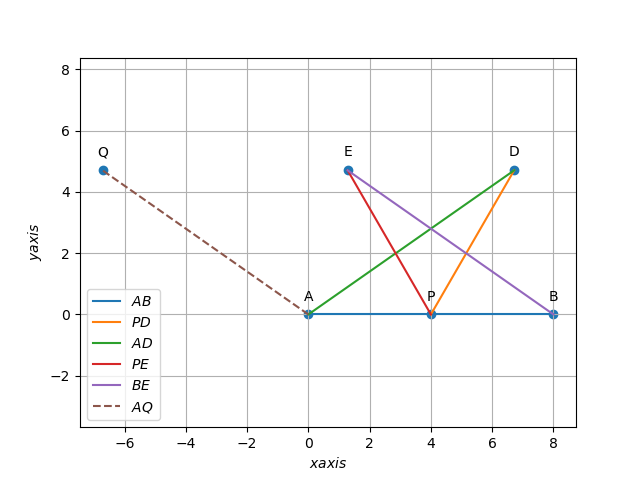
\includegraphics[scale=0.4]{fig.png} 
\caption{}
\end{figure}
\section{Code}
*Verify the above proofs in the following code.\\
\framebox{
\url{https://github.com/Susi9121/FWC/tree/main/matrix/line}}	
\bibliographystyle{ieeetr}
\end{document}
\fi

\item Show that the points A (1, -2, -8), B (5, 0, -2) and C (11, 3, 7) are collinear, and find the ratio in which B divides AC.\\
\end{enumerate}
